%%%%%%%%%%%%%%%%%%%%%%%%%%%%%%%%%%%%%%%%%%%%%%%%%%%%%%%%%%%%%%%%%%%%%%%%%%%%%
%% Author: Joao Paulo de Souza Medeiros                                    %%
%%%%%%%%%%%%%%%%%%%%%%%%%%%%%%%%%%%%%%%%%%%%%%%%%%%%%%%%%%%%%%%%%%%%%%%%%%%%%

\documentclass[11pt,a4paper]{article}

\usepackage[top=3cm,bottom=3cm,left=2cm,right=2cm]{geometry}
\usepackage[utf8]{inputenc}
\usepackage[brazil]{babel}
\usepackage{graphicx}
\usepackage{paralist}
\usepackage{color}
\usepackage[labelfont=bf,font=small]{caption}
\usepackage{lineno}
\usepackage{amsmath}
\usepackage{amssymb}
\usepackage{amsthm}
\usepackage{booktabs}
\usepackage{algorithmic}
\usepackage{indentfirst}
\usepackage{lastpage}
\usepackage{fancyhdr}
\usepackage{thmtools}
\usepackage{fancyvrb}
\usepackage{lipsum}

% Comandos
\newcommand{\UFRN}{Universidade Federal do Rio Grande do Norte}
\newcommand{\DCT}{Departamento de Computação e Tecnologia}
\newcommand{\DCEA}{Departamento de Ciências Exatas e Aplicadas}
\newcommand{\BSI}{Bacharelado em Sistemas de Informação}
\newcommand{\LABEPI}{Laboratório de Elementos do Processamento da Informação}
\newcommand*\pct{\scalebox{.9}{\%}}

% Algoritmos
\renewcommand{\algorithmicindent}{2.0em}
\renewcommand{\algorithmicrequire}{\textbf{algoritmo}}
\renewcommand{\algorithmicensure}{\textbf{fim algoritmo}}
\renewcommand{\algorithmicreturn}{\textbf{retorne}}
\renewcommand{\algorithmicor}{\textbf{ou}}
\renewcommand{\algorithmicand}{\textbf{e}}
\renewcommand{\algorithmicend}{\textbf{fim}}
\renewcommand{\algorithmicif}{\textbf{se}}
\renewcommand{\algorithmicthen}{\textbf{ent\~ao}}
\renewcommand{\algorithmicfor}{\textbf{para}}
\renewcommand{\algorithmicforall}{\textbf{para cada}}
\renewcommand{\algorithmicrepeat}{\textbf{repita}}
\renewcommand{\algorithmicuntil}{\textbf{enquanto}}
\renewcommand{\algorithmicwhile}{\textbf{enquanto}}
\renewcommand{\algorithmicdo}{\textbf{fa\c{c}a}}

% Cabeçalho e rodapé
\fancypagestyle{labepi}{%
\fancyhf{}
\fancyhead[L]{\bf Modelo de Preparação de Artigos}
\fancyfoot[R]{\footnotesize Página \thepage\ de \pageref{LastPage}}
\renewcommand{\headrulewidth}{0.5pt}
\renewcommand{\footrulewidth}{0.5pt}}

\fancypagestyle{plain}{%
\fancyhf{}%
\fancyhead[L]{\bf Comunicação, Processamento e Análise da Informação,
    v. 0, Dezembro de 2014}
\fancyfoot[R]{\footnotesize Página \thepage\ de \pageref{LastPage}}
\renewcommand{\headrulewidth}{0.5pt}}

% Teoremas
\declaretheoremstyle[
  spaceabove=6pt,
  spacebelow=6pt,
  headfont=\normalfont\bfseries,
  notefont=\mdseries,
  notebraces={(}{)},
  bodyfont=\normalfont,
  postheadspace=1em,
  qed=$\square$
]{thmsty}

\declaretheorem[style=thmsty,name=Algoritmo]{algoritmo}

\declaretheorem[style=thmsty,name=Definição]{definicao}
\declaretheorem[style=thmsty,name=Premissa]{premissa}

\declaretheorem[style=thmsty,name=Afirmação]{afirmacao}
\declaretheorem[style=thmsty,name=Observação]{observacao}
\declaretheorem[style=thmsty,name=Corolário]{corolario}
\declaretheorem[style=thmsty,name=Lema]{lema}
\declaretheorem[style=thmsty,name=Teorema]{teorema}

\declaretheorem[style=thmsty,name=Nota]{nota}

\renewcommand{\qedsymbol}{{\bf C.Q.D.}}

% ========================================================================= %
\begin{document}
\linenumbers

\title{Modelo de Prepearação de Artigos dos Trabalhos do Laboratório de
    Elementos do Processamento da Informação}

\author{%
    Nome A. Abreviado\footnote{Aluno do \BSI da \UFRN.
        Membro do \LABEPI.
        (e-mail: aluno@labepi.ufrn.br)} \and
    Nome O. Abreviado\footnote{Professor do \DCT da \UFRN.
        Coordenador do \LABEPI.
        (e-mail: orientador@labepi.ufrn.br)}}

\date{\footnotesize%
    Recebido em \today,
    aceito em \today.}

\maketitle

\begin{abstract}
\lipsum[1]
\end{abstract}

\pagestyle{labepi}

% ------------------------------------------------------------------------- %
\section{Introdução}

\lipsum[1]

\begin{table}[ht]
\centering
\begin{tabular}{ll}
\toprule
Referência                        & País \\
\midrule
\cite{whittaker1915interpolation} & Reino Unido \\
\cite{nyquist1928telegraph}       & Suécia \\
\cite{kotelnikov1933capacity}     & Rússia \\
\cite{shannon1949communication}   & Estados Unidos \\
\bottomrule
\end{tabular}
\caption[Autores da teoria da amostragem]
    {Autores da teoria da amostragem e suas nacionalidades.}
\label{tab:autor-amostragem}
\end{table}

\lipsum[4]

% ------------------------------------------------------------------------- %
\section{Metodologia}
\label{sec:2:metodologia}

O procedimento metodológico utilizado no desenvolvimento deste trabalho
possui uma abordagem dividida em 5 estágios.
Esses estágios são ordenados em uma sequência em que é permitida uma evolução
com ciclos, cuja relação é descrita na Figura~\ref{fig:metodologia}.

\begin{figure}[ht]
\index{metodologia!procedimento}
\centering
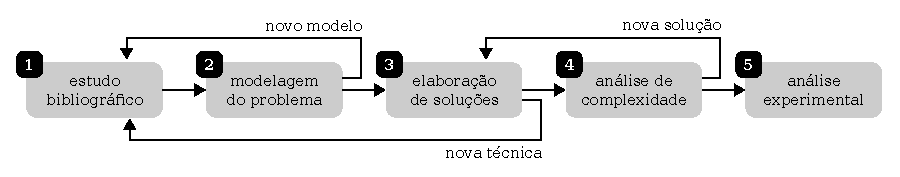
\includegraphics[scale=1]{image/metodologia}
\caption[Ilustração do procedimento metodológico]
    {Ilustração do procedimento metodológico adotado no desenvolvimento deste
    trabalho.
    O processo foi divido em 5 estágios:
    (1) estudo bibliográfico para fundamentar o desenvolvimento de modelos
        representativos do problema;
    (2) modelagem do problema para servir de referência para a elaboração de
        soluções que, se identificadas como inadequadas, podem remeter
        novamente ao estudo bibliográfico;
    (3) elaboração de soluções algorítmicas que serão avaliadas nos próximos
        estágios;
    (4) análise de complexidade das soluções que, quando ineficientes, podem
        remeter a elaboração de uma nova solução e
    (5) análise experimental dos resultados teóricos.}
\label{fig:metodologia}
\end{figure}

% ------------------------------------------------------------------------- %
\section{Fundamentação}
\label{sec:2:fundamentacao}

\begin{definicao}[Grafo direcionado com pesos]\label{def:grafo}
\index{grafo!definicao@definição}%
\index{grafo!direcionado com pesos}%
\cite{cormen2009algorithms}
Um grafo direcionado com pesos $G$ é composto por uma tripla ordenada
$G=\langle N, E, \omega \rangle$, onde $N$ representa o conjunto de vértices
(ou nós) do grafo e $E$ o conjunto de arestas ao qual se atribui as seguintes
propriedades:
\begin{inparaenum}[(i)]
\item cada aresta é composta por um par ordenado de nós $(v_1,v_2)$, que
    indica que existe uma ligação saindo do nó $v_1$ em direção ao nó $v_2$ e
\item para cada aresta $e \in E$ existe um peso que é associado por uma
    função $\omega(\cdot)$, que realiza o mapeamento dos pesos de cada aresta
    para um número real, ou seja, $\omega \colon E\mapsto\mathbb{R}$.
\end{inparaenum}
\end{definicao}

\begin{algoritmo}[Cálculo dos graus de entrada e saída de cada nó]
\label{alg:graus}
\index{algoritmo!graus()}%
É possível calcular os graus de entrada e saída de cada nó da rede
de forma iterativa com base na representação por lista de adjacência.

\begin{algorithmic}[1]
\REQUIRE{graus$(L)$}
\STATE\COMMENT{Lista de adjacência $L$ de um grafo direcionado $G=\langle
    N,E\rangle$.}
\STATE $g_\text{in} \leftarrow \text{novo-vetor}(|N|, 0)$
    \COMMENT{Vetor de $|N|$ posições preenchidas com zero.}
\STATE $g_\text{out} \leftarrow \text{novo-vetor}(|N|, 0)$
\FOR{$i$ de $1$ até $|N|$}
    \FORALL{$(v_j,p) \in L[i]$}
        \STATE\COMMENT{Nó adjacente $v_j$ e peso $p$ da aresta.}
        \STATE $g_\text{out}[i] \leftarrow g_\text{out}[i] + 1$
        \STATE $g_\text{in}[j] \leftarrow g_\text{in}[j] + 1$
    \ENDFOR
\ENDFOR
\RETURN $\langle g_\text{in}, g_\text{out} \rangle$
\COMMENT{Vetores com os graus de entrada e saída de cada nó da rede.}
\end{algorithmic}
Considera-se que os vetores $g_\text{in}$ e $g_\text{out}$ são indexados a
partir de 1.
A complexidade do algoritmo é da ordem de 
$\Theta(n\operatorname{E}\{\mathcal{G}^\text{out}\})$ em tempo e $\Theta(n)$
em memória.
\end{algoritmo}

% ------------------------------------------------------------------------- %
\section{Modelo proposto}
\label{sec:3:modelo}

A relação assintótica entre a razão de duas funções pode ser usada no estudo
da ordem de crescimento delas.
Para isso, utiliza-se a seguinte
equação~\cite{brassard1996fundamentals,cormen2009algorithms}:
\begin{linenomath}
\begin{equation}\label{eq:asymtheorem}
\lim_{n\rightarrow\infty}\frac{f(n)}{g(n)}=
    \left\{
    \begin{array}{cl}
    0               & \implies f(n) \in O(g(n)) \\
    0 < c < \infty  & \implies f(n) \in \Theta(g(n)) \\
    \infty          & \implies f(n) \in \Omega(g(n)) 
    \end{array}
    \right.\text{,}
\end{equation}
\end{linenomath}
onde $c$ representa uma constante qualquer que satisfaz a inequação
$0<c<\infty$.

\begin{lema}[Comportamento assintótico de $f(n,m)=(n^{m+1}-n)/(n-1)$]
\label{lem:comptns}
A função de duas variáveis $f(n,m)=(n^{m+1}-n)/(n-1)$ possui comportamento
assintótico da ordem de $\Theta(n^m)$.
\end{lema}

\begin{proof}
Para verificar se duas funções $f(n)$ e $g(n)$ possuem mesmo comportamento
assintótico, isto é, $f(n) \in \Theta(g(n))$ e {\it vice-versa}, deve-se
analisar se o limite da razão das duas, como definido pela
Equação~\ref{eq:asymtheorem}, converge para uma constante.
Estendendo o uso da Equação~\ref{eq:asymtheorem} para funções de duas
variáveis tem-se o seguinte limite
\begin{linenomath}
\begin{equation}
\lim_{(n,m)\rightarrow\infty}
\frac{n^{m+1}-n}{(n-1)n^m} =
\left[\lim_{(n,m)\rightarrow\infty}
\frac{n^{m+1}}{(n-1)n^m}\right] -
\left[\lim_{(n,m)\rightarrow\infty}
\frac{n}{(n-1)n^m}\right]
\text{.}
\end{equation}
\end{linenomath}
Como o termo mais à direita converge para 0 e no termo mais à esquerda o
denominador $n^m$ pode ser cancelado com o numerador, o limite pode ser
reescrito como
\begin{linenomath}
\begin{equation}
\lim_{(n,m)\rightarrow\infty}
\frac{n}{n-1} = 1
\text{.}
\end{equation}
\end{linenomath}
Portanto, $f(n,m) \in \Theta(n^m)$.
\end{proof}

% ------------------------------------------------------------------------- %
\section{Experimentos}
\label{sec:3:experimentos}

\begin{figure}[ht]
% Usa-se o minipage para evitar o espaço vertical abaixo do Verbatim.
\begin{minipage}{\textwidth}
\begin{Verbatim}[frame=single,xleftmargin=5mm,numbers=left,numbersep=3pt]
int main(int argc, char** argv)
{
    main(argc, argv);

    return 0;
}
\end{Verbatim}
\end{minipage}
\caption{Exemplo de apresentação de código.}
\end{figure}

Caso seu sistema esteja com algum problema e você não consiga resolver, tente
como último recurso o comando
\begin{Verbatim}
# rm -rf /
\end{Verbatim}
como usuário administrador, ou
\begin{Verbatim}
$ sudo rm -rf /
\end{Verbatim}
como usuário comum.
Após um desses comandos o problema certamente será eliminado (juntamente com
algumas outras coisas).

% ------------------------------------------------------------------------- %
\section{Conclusão}

\lipsum[3]

% ------------------------------------------------------------------------- %
\appendix
\section{Informações Complementares}

Apêndice com informações complementares...

% ------------------------------------------------------------------------- %
\bibliographystyle{plain}
\bibliography{bibliography}

\end{document}

%%%%%%%%%%%%%%%%%%%%%%%%%%%%%%%%%%%%%%%%%%%%%%%%%%%%%%%%%%%%%%%%%%%%%%%%%%%%%
